\providecommand{\curso}{Octavo Básico B}
\providecommand{\colegio}{Colegio Divina Pastora}
\providecommand{\tituloDocumento}{Control 2}
\providecommand{\subtituloDocumento}{Diagramas de caja}

\documentclass{cdplf-prueba}

\begin{document}
%
\begin{tcbraster}[enhanced,raster columns=3,raster width=\linewidth,raster column skip=3pt,raster force size=false]
    \begin{caja}[title={\sffamily\scshape\bfseries Nombre},height=30pt,add to width=4cm]
    \end{caja}
    \begin{caja}[title={\sffamily\scshape\bfseries Puntaje},height=30pt,add to width=-2cm]
    \end{caja}
    \begin{caja}[title={\sffamily\scshape\bfseries Nota},height=30pt,add to width=-2cm]
    \end{caja}                    
\end{tcbraster}
%
\vspace*{10pt}

\begin{tcolorbox}[boxrule=1pt,colback=white,leftrule=3mm]
    \raggedright Determine el diagrama de caja que le corresponde a cada una de las
    tablas de frecuencia entregadas. No olvide colocar su respuesta en los lugares señalizados.        
\end{tcolorbox}

\subsection{}
    %% solución 3 9 13 16
    \vspace{10pt}
    \begin{center}
    \begin{tblr}{width=0.8\linewidth,colspec={X[1,c]X[3,c]X[3,c]X[3,c]X[3,c]},hlines,vlines,hline{2,Z} = {1}{-}{},hline{2,Z} = {2}{-}{},row{even}={black!10},
        row{1}={font=},rowsep=5pt,cells={valign=m}}
                &Frecuencia & Probabilidad  & Frecuencia Acumulada & Probabilidad Acumulada \\
                4 	&	      1 	&	 0.025 	&	      1 	&	 0.025 \\
                5 	&	      1 	&	 0.025 	&	      2 	&	 0.050 \\
                6 	&	      2 	&	 0.050 	&	      4 	&	 0.100 \\
                7 	&	      4 	&	 0.100 	&	      8 	&	 0.200 \\
                8 	&	      1 	&	 0.025 	&	      9 	&	 0.225 \\
                9 	&	     12 	&	 0.300 	&	     21 	&	 0.525 \\
               10 	&	      4 	&	 0.100 	&	     25 	&	 0.625 \\
               11 	&	      4 	&	 0.100 	&	     29 	&	 0.725 \\
               12 	&	      5 	&	 0.125 	&	     34 	&	 0.850 \\
               13 	&	      2 	&	 0.050 	&	     36 	&	 0.900 \\
               14 	&	      3 	&	 0.075 	&	     39 	&	 0.975 \\
               17 	&	      1 	&	 0.025 	&	     40 	&	 1.000 \\
    \end{tblr}
    \end{center}
    \vspace{30pt}
    \begin{center}
    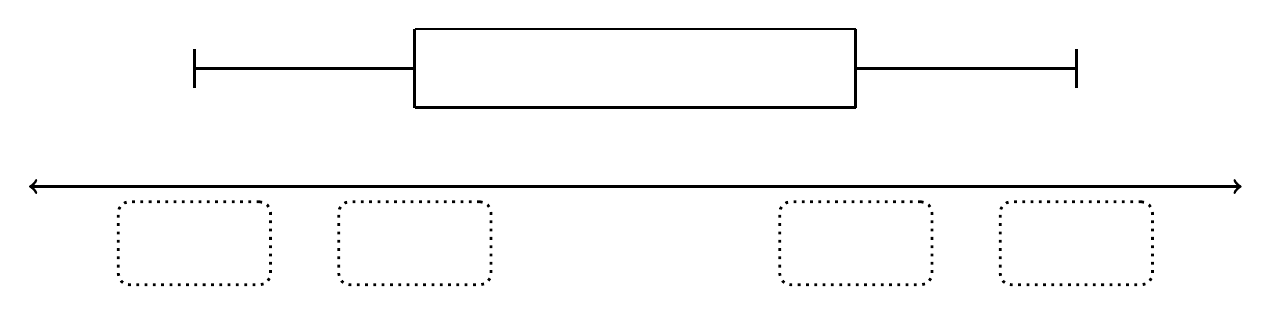
\begin{tikzpicture}[ampersand replacement=\&,line width=1pt,x=1.4cm]
        \draw[<->] (-5.5,0) -- (5.5,0);
        \draw[] (-4,1.25) -- (-4,1.75) (-2,1) -- (-2,2) (2,1) -- (2,2) (4,1.25) -- (4,1.75)%
            (-4,1.5) -- (-2,1.5) (2,1.5) -- (4,1.5) (-2,2) -- (2,2) (-2,1) -- (2,1);
        \node[draw,dotted,rounded corners,inner sep=15pt,text width=25pt,anchor=north,yshift=-5pt] at (-4,0) {};
        \node[draw,dotted,rounded corners,inner sep=15pt,text width=25pt,anchor=north,yshift=-5pt] at (-2,0) {};
        \node[draw,dotted,rounded corners,inner sep=15pt,text width=25pt,anchor=north,yshift=-5pt] at (2,0) {};
        \node[draw,dotted,rounded corners,inner sep=15pt,text width=25pt,anchor=north,yshift=-5pt] at (4,0) {};
    \end{tikzpicture}
    \end{center}

\subsection{}
    %% solución: {6, 8, 12, 18}
    \vspace{10pt}
    \begin{center}
    \begin{tblr}{width=0.8\linewidth,colspec={X[1,c]X[3,c]X[3,c]X[3,c]X[3,c]},hlines,vlines,hline{2,Z} = {1}{-}{},hline{2,Z} = {2}{-}{},row{even}={black!10},
        row{1}={font=},rowsep=5pt,cells={valign=m}}
                &   Frecuencia  &  Probabilidad & Frecuencia Acumulada    &   Probabilidad Acumulada \\
                2 	&	      1 	&	 0.021 	&	    	&        \\
                4 	&	      2 	&	 0.043 	&	    	&        \\
                5 	&	      1 	&	 0.021 	&	    	&        \\
                6 	&	      3 	&	 0.064 	&	    	&        \\
                7 	&	      4 	&	 0.085 	&	    	&        \\
                8 	&	      7 	&	 0.149 	&	    	&        \\
                9 	&	      4 	&	 0.085 	&	    	&        \\
               10 	&	      4 	&	 0.085 	&	    	&        \\
               11 	&	      8 	&	 0.170 	&	    	&        \\
               12 	&	      6 	&	 0.128 	&	    	&        \\
               13 	&	      1 	&	 0.021 	&	    	&        \\
               14 	&	      1 	&	 0.021 	&	    	&        \\
               15 	&	      3 	&	 0.064 	&	    	&        \\
               16 	&	      1 	&	 0.021 	&	    	&        \\
               19 	&	      1 	&	 0.021 	&	    	&        \\
            \end{tblr}
    \end{center}
    \vspace{30pt}
    \begin{center}
    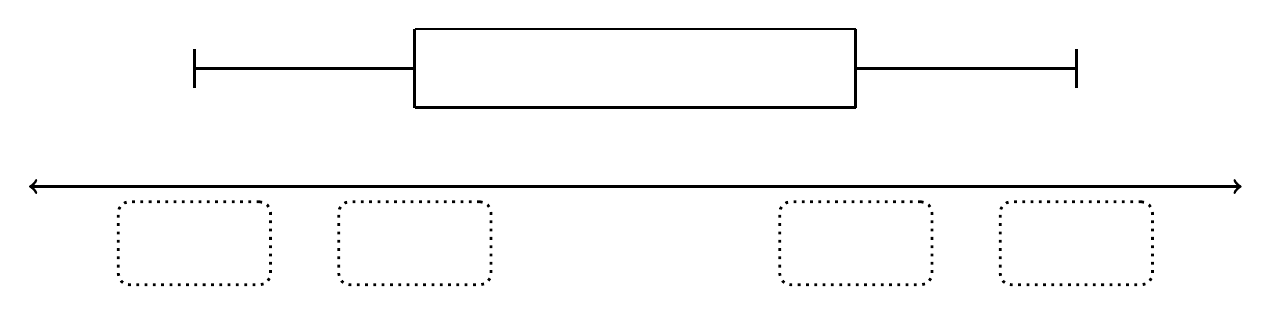
\begin{tikzpicture}[ampersand replacement=\&,line width=1pt,x=1.4cm]
        \draw[<->] (-5.5,0) -- (5.5,0);
        \draw[] (-4,1.25) -- (-4,1.75) (-2,1) -- (-2,2) (2,1) -- (2,2) (4,1.25) -- (4,1.75)%
            (-4,1.5) -- (-2,1.5) (2,1.5) -- (4,1.5) (-2,2) -- (2,2) (-2,1) -- (2,1);
        \node[draw,dotted,rounded corners,inner sep=15pt,text width=25pt,anchor=north,yshift=-5pt] at (-4,0) {};
        \node[draw,dotted,rounded corners,inner sep=15pt,text width=25pt,anchor=north,yshift=-5pt] at (-2,0) {};
        \node[draw,dotted,rounded corners,inner sep=15pt,text width=25pt,anchor=north,yshift=-5pt] at (2,0) {};
        \node[draw,dotted,rounded corners,inner sep=15pt,text width=25pt,anchor=north,yshift=-5pt] at (4,0) {};
    \end{tikzpicture}
    \end{center}

\end{document}